%%%%           %%%%
%%%% ANÁLISIS  %%%%
%%%%           %%%%

\chapter{Análisis}
\label{chap:analisis}

\lettrine{E}{n} este capítulo se tratará los aspectos del análisis de la aplicación. Se verán los requisitos, funcionales y no funcionales, los casos de uso y por último se presentarán los modelos de los documentos tratados.

\section{Actores y casos de uso}

Un caso de uso describe una interacción entre un rol y el sistema. O cómo es utilizado por un usuario para completar una tarea u alcanzar un objetivo. En el Diagrama \ref{fig:casos-de-uso} se presentan los casos de uso de la aplicación. 

Existen dos actores que interactúan con la aplicación, un Sistema Externo y una Base de Datos:

\begin{itemize}
	\item \textbf{Sistema Externo}: la aplicación está diseñada para comunicarse con el Sistema Externo mediante invocación directa de comandos o bien un por medio del motor que gestiona el procesamiento. Si bien mediante comandos un usuario podría solicitar la ejecución de trabajos, el objetivo principal es ser un backend en disposición de ser empleado por otros sistemas.
	\item \textbf{Base de Datos}: este agente es consultado para la obtención de datos de identificación de los documentos.
\end{itemize}

Se presentan a continuación los casos de uso de forma detallada:

\begin{itemize}
	\item \textbf{CU-01} - Registrar nuevo trabajo
	\begin{itemize}
		\item \textbf{Descripción}: el Sistema Externo solicita la generación de un nuevo identificador para un trabajo.
		\item \textbf{Precondición}: el motor está operativo y esperando trabajo.
		\item \textbf{Postcondición}: se genera el identificador y se ha creado la ruta correspondiente en el sistema de ficheros para el trabajo.
	\end{itemize}
\item \textbf{CU-02} - Generar JSON
	\begin{itemize}
		\item \textbf{Descripción}: el sistema externo facilita un lote de ficheros y un identificador del trabajo para comenzar su tratamiento.
		\item \textbf{Precondición}: el identificador debió ser creado previamente.
		\item \textbf{Postcondición}: los resultados de la operativa están disponibles en las rutas previstas.
\end{itemize}
\item \textbf{CU-03} - Generar imágenes
	\begin{itemize}
		\item \textbf{Descripción}: el sistema genera imágenes para cada una de las páginas de los documentos.
		\item \textbf{Precondición}: se han podido recuperar los PDF individuales y se encuentran en las rutas previstas.
		\item \textbf{Postcondición}: existe un fichero para cada página de cada documento en la ruta de salida.
\end{itemize}
\item \textbf{CU-04} - Informar error
	\begin{itemize}
		\item \textbf{Descripción}: en caso de problemas durante el procesamiento se informa al sistema externo del error ocurrido.
		\item \textbf{Precondición}: sucede una condición de error en el sistema.
		\item \textbf{Postcondición}: dependiendo del tipo de error el engine consigue finalizar el procesamiento o se finaliza si no es posible recuperarse del error.
\end{itemize}
\item \textbf{CU-05} - Relacionar documento y plantilla
	\begin{itemize}
		\item \textbf{Descripción}: a partir de los datos extraídos del documento en curso se consigue identificar la plantilla correcta para la generación de su lenguaje intermedio y su posterior proceso de parseo. La búsqueda del identificador se solicita a una base de datos externa.
		\item \textbf{Precondición}: los datos extraídos son de la suficiente calidad para contener el identificador del documento.
		\item \textbf{Postcondición}: se genera un fichero con el identificador único de la plantilla.Precondición
\end{itemize}
\item \textbf{CU-06} - Identificar la finalización
	\begin{itemize}
		\item \textbf{Descripción}: al finalizar el procesamiento del lote de ficheros se genera una marca de finalización del trabajo.
		\item \textbf{Precondición}: se completa el tratamiento de todos los documentos sin errores mayores.
		\item \textbf{Postcondición}: la marca de finalización está en la ruta preestablecida del sistema de ficheros.
\end{itemize}

\end{itemize}

\begin{figure}[hp!]
	\centering
	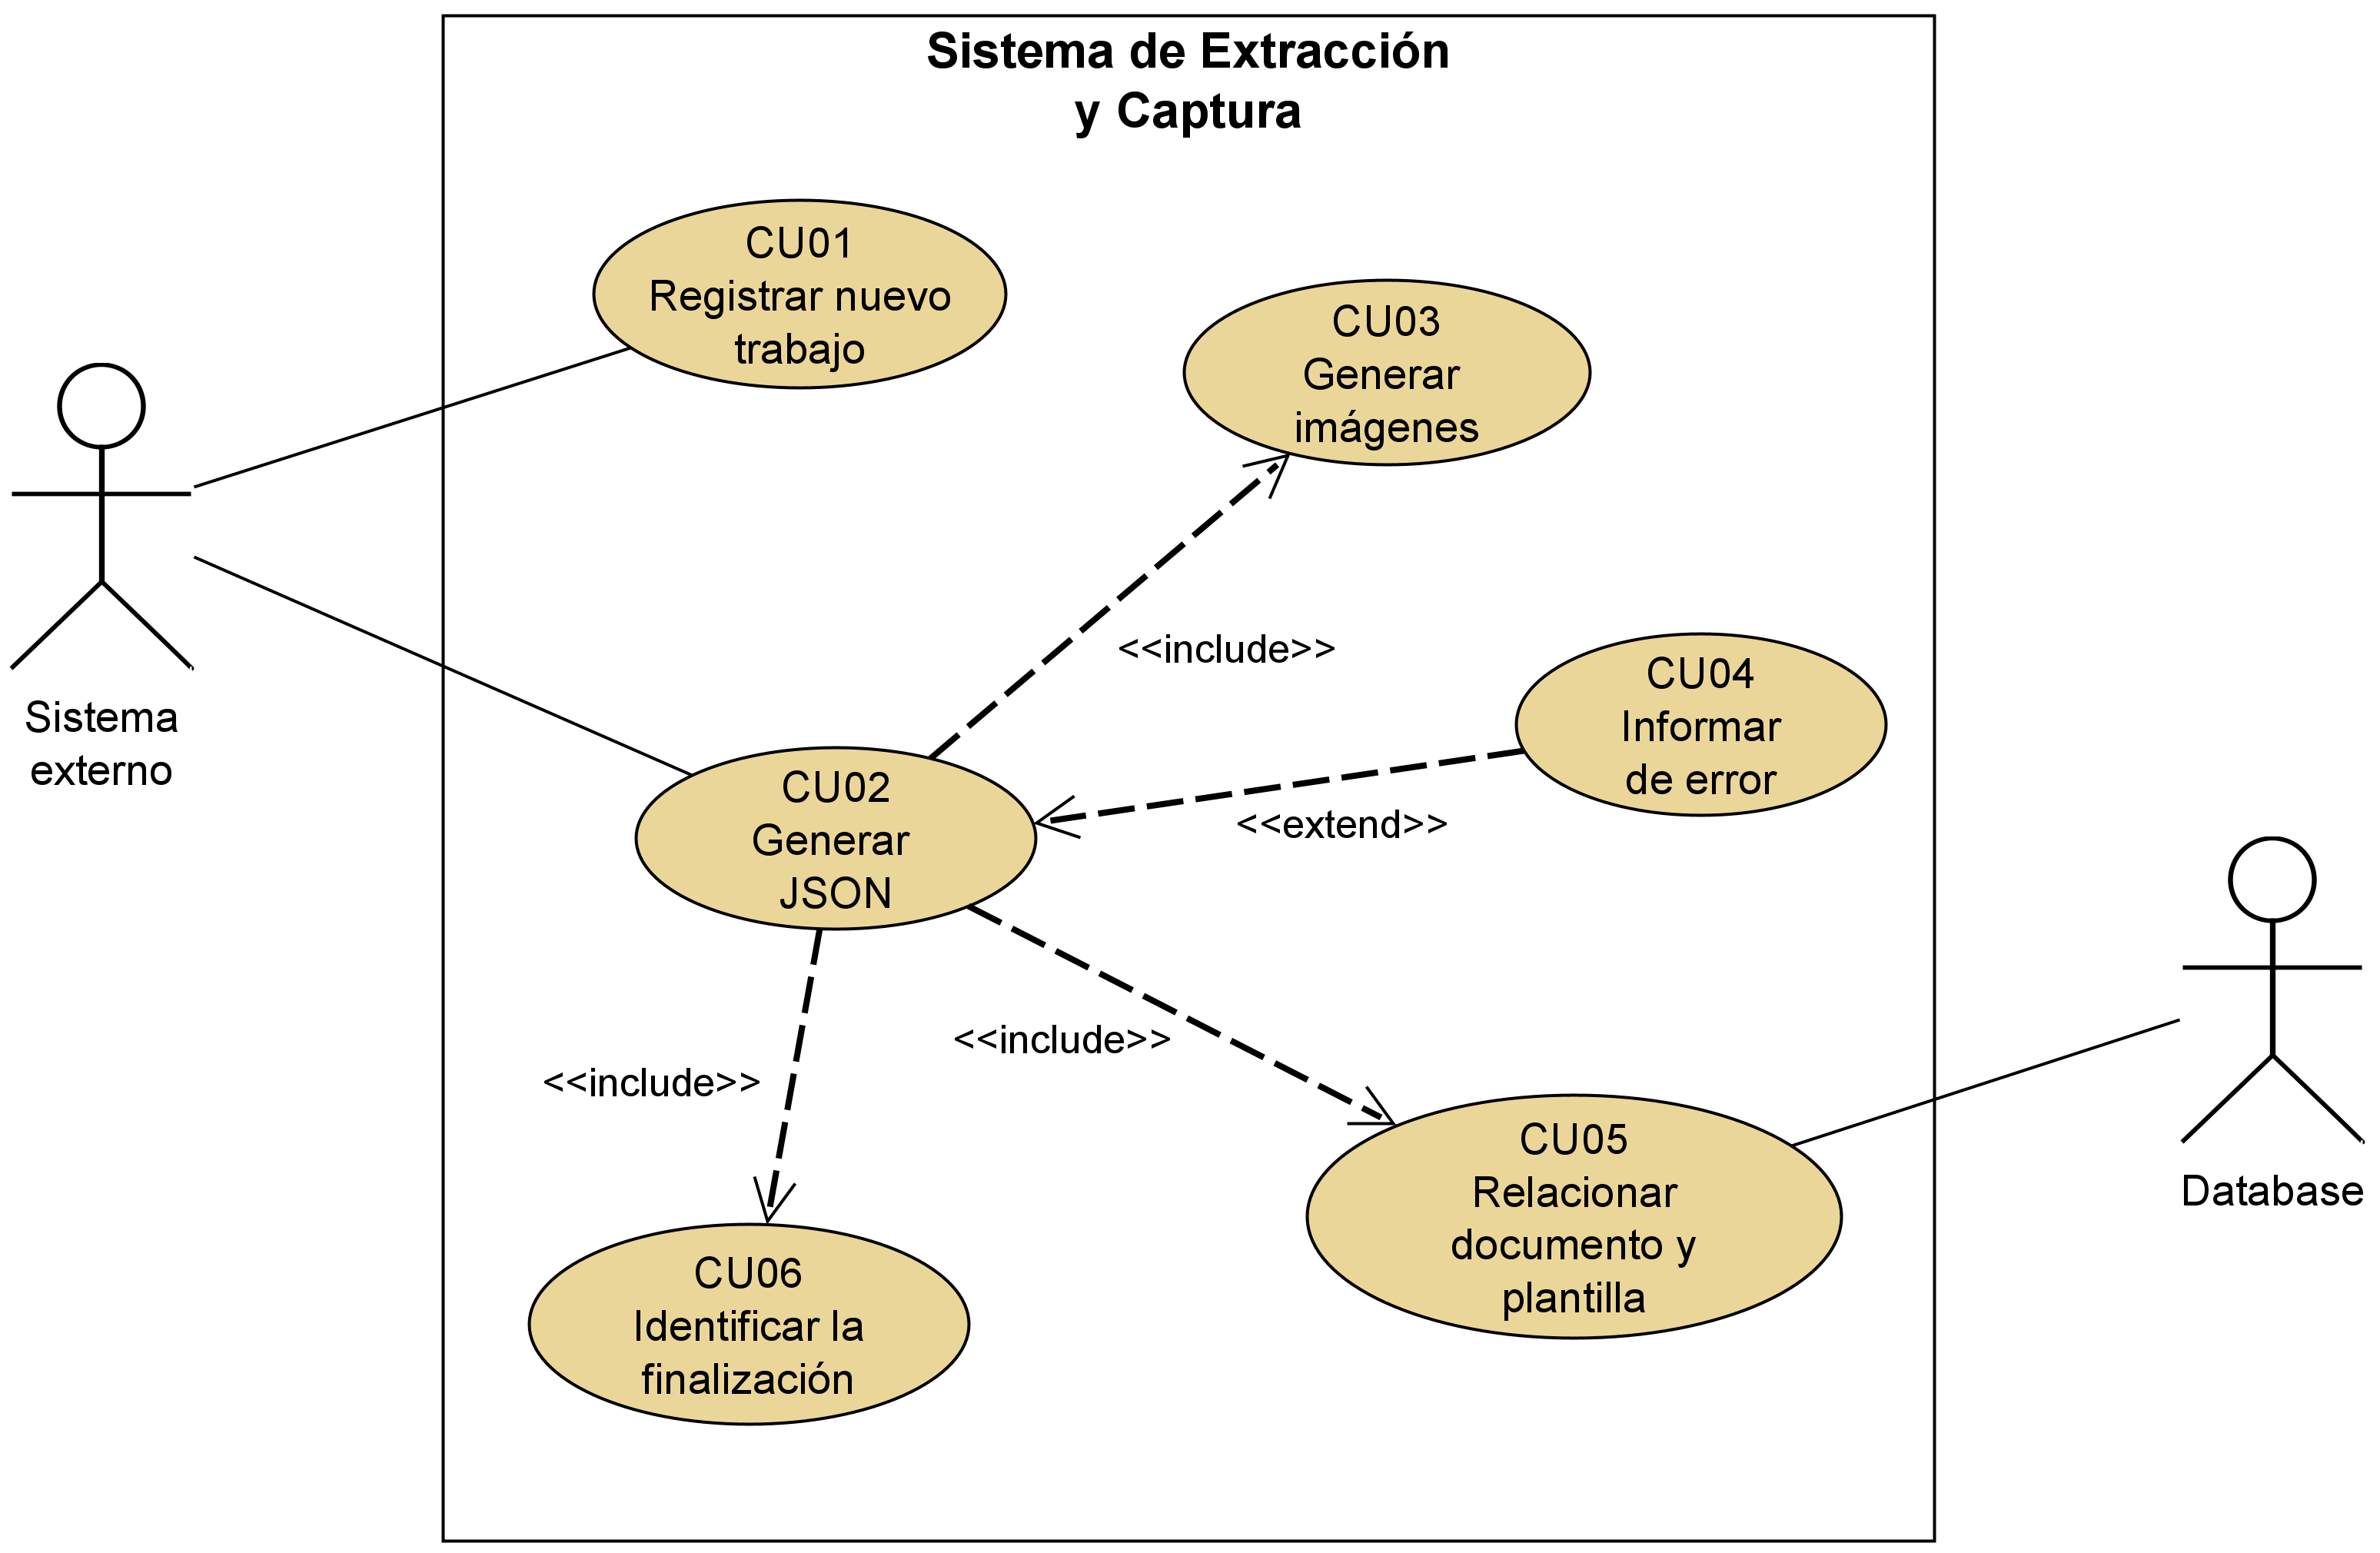
\includegraphics[width=1.0\textwidth]{imaxes/g-analisis/casos-uso.png}
	\caption{Casos de uso del software}
	\label{fig:casos-de-uso}
\end{figure}

\section{Requisitos funcionales}

Estos son los requisitos funcionales que la aplicación debe soportar:

\begin{itemize}
	\item Obtención de un identificador único de un trabajo, con anterioridad a la ejecución del mismo.
	\item Generación una salida en formato estructurado para cada documento suministrado y reconocido en el sistema.
	\item Creación de imágenes de las páginas individuales de cada uno de los documentos.
	\item Creación de una marca de finalización para cada trabajo completado.
\end{itemize}


\section{Requisitos no funcionales}

Se exponen ahora los requisitos no funcionales de la aplicación:

\begin{itemize}
	\item La entrada podrá contener uno o más ficheros para su tratamiento en el mismo lote.
	\item Procesamiento de los modelos de imagen y texto de forma transparente al usuario.
	\item La salida de una ejecución debe facilitar los resultados de forma individualizada para cada documento.
	\item Se deben poder identificar las líneas individuales de contenido en  las tablas presentes en los documentos.
\end{itemize}

\section{Sobre los documentos}
\label{sec:sobre-los-documentos}

Para proceder a la inclusión de un nuevo modelo de documento hay que entender como está constituido, qué información ofrece, si tienen tablas y como se utilizan en el modelo. En el caso de documentos con más de una página, hay que determinar si en cada una se repiten los mismos elementos o por el contrario, cualquiera de ellas, ya sea la primera, las páginas intermedias o la final, tienen características propias, como puede ser la extensión de las regiones o posición de las mismas. Este análisis de los modelos tratados en el trabajo se presenta a continuación. Para facilitar la compresión de las características se han incluido imágenes completas de algunos documentos en el Apéndice \ref{chap:adicional-1}.

Durante la generación de código y posterior tratamiento del lenguaje intermedio, una de las dificultades habituales consiste en localizar las líneas individuales de contenido. Es frecuente que alguna de las columnas tenga datos en varias filas físicas que refieran a una misma línea de contenido, tal como se muestra en la Imagen \ref{fig:una-linea-lógica-varias-fisicas}. Para un resultado satisfactorio, hay que aprovechar alguna característica que permita esta separación de tal manera que los datos de filas distintas no se mezclen entre si. Esto sucedería si simplemente se generase un código intermedio donde se colocase el texto de forma secuencial considerando únicamente sus coordenadas.

\begin{figure}[hp!]
    \centering
    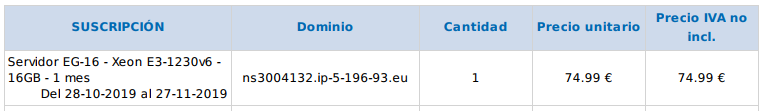
\includegraphics[width=0.9\textwidth]{imaxes/g-analisis/varias-lineas-en-una.png}
    \caption{Una línea lógica utilizando varias líneas físicas}
    \label{fig:una-linea-lógica-varias-fisicas}
\end{figure}

\subsection{Prodware}

Los documentos presentan un layout fijo que se repite en todos los ejemplares. En la parte superior se encuentran los datos de emisor y receptor. Aunque los cuadros no están dibujados, las dimensiones y localización son constantes. Más abajo aparece una primera tabla con una fila para la cabecera y otra fila para la información. La tabla principal de datos tiene tres columnas relativas a la fecha, descripción e importe. En algunos documentos las líneas de la columna \emph{Descripción} ocupan varias líneas físicas. Para la identificación de las líneas de contenido se pueden utilizar las fechas de la primera columna dado que aunque la descripción ocupe varias líneas físicas, las fechas contienen espacios en las segundas o terceras líneas. En la parte inferior están las tablas con información de resumen del documento. Esta información de resumen emplea las mismas dimensiones y espacios en todos los documentos de la muestra. A mayores, dos casos son diferentes en cuanto a que no presentan las líneas de las tablas. No obstante, dado que no es necesario recurrir a la Transformada de Hough para este modelo y que las posiciones se mantienen sin cambios, no supone diferencia para el tratamiento.
 
\subsection{Adobe}

Los ejemplares de facturas de Adobe presentan todos dos páginas. No obstante la segunda página carece de contenido relevante, ya que replica los datos de resumen de la factura, que aparecen idénticos en la primera página. Por tanto, las regiones definidas en la plantilla omitirán estas segundas páginas en este modelo.
Todos los casos presentan el mismo layout, con idéntica ubicación para las tablas, celdas y datos individuales. En la parte superior de los documentos aparece la información de identificación del cliente y emisor, a la izquierda, y los datos relativos a la factura, en la parte derecha.
La tabla principal contiene seis columnas. Tras la revisión de los casos no es posible determinar si existen líneas de contenido que se extiendan más allá de una línea física de la tabla.
En la parte inferior se encuentran los datos de resumen como importe, tipo de IVA aplicado y totales.

\subsection{OVH}

Este modelo es el que presenta más variabilidad en su construcción. En la parte superior de la primera página siempre aparece el logotipo de la empresa, a la izquierda, y los datos de identificación de la factura, a la derecha. La información de identificación si que ocupa el mismo tamaño y ubicación en todas las primeras páginas. Para la identificación de las filas de las tablas se utilizará la Transformada de Hough porque existen casos donde el contenido ocupa varias líneas, pero las tablas están perfectamente delimitadas. Por otra parte, las tablas no tienen longitud fija, sino que se extienden tanto como sea necesario para alojar los datos, extendiéndose incluso páginas enteras. Esto quiere decir que no se puede utilizar el tamaño como indicador del final. El interior de las tablas es siempre el mismo. Hay 5 columnas y una primera fila de cabecera con los nombres de las columnas. Encima de la primera fila hay un texto que categoriza la partida de gasto. La última fila de cada tabla contiene la suma del importe de las filas de la tabla precedido de la etiqueta \emph{SUBTOTAL}. Cuando una de las tablas llega hasta el final de la página, siempre se respeta una altura máxima. Esto quiere decir que las regiones se pueden definir utilizando este máximo.

En la última página, si tienen más de una, o en la parte final si solo tienen una, aparece siempre un resumen con los importes. Tras el resumen, existe siempre una línea de texto \emph{Factura pagadera en el momento de la recepción}. La ubicación de esta última tabla puede ser calculada a partir de los textos de la cabecera y de la última línea.

\subsection{AC}

Los documentos de esta empresa pueden tener una o varias páginas. El caso con varias páginas respeta los tamaños y posiciones de los datos. En la parte superior se encuentra el logotipo y datos de la empresa, a la izquierda, y los datos identificativos del cliente, a la derecha. Debajo de la identificación hay regiones simples con los datos identificativos de la factura. En tercer lugar se encuentra la tabla principal de datos que contienen doce columnas. Si bien no se dan casos donde una línea de contenido ocupe más que una línea física, en este modelo algunos datos de columnas diferentes se presentan muy próximos entre si. Aunque el final de la tabla principal no está dibujado, se puede observar que todas las páginas respetan un tamaño máximo que será el punto hasta el que se extienda la región. En la aparte inferior se encuentran los datos de resumen de la factura, con importes desglosados por tipo de IVA y los totales.
 
\subsection{Tipos de regiones}

Vistos los documentos, se concluye que las regiones existentes se pueden categorizar en cuatro tipos y variantes para poder tratar todos los escenarios:

\begin{enumerate}
	\item Tablas simples de dos columnas, cabecera en la columna de la derecha y $m$ filas. Estas son las regiones \verb|R1|, tal como se ejemplifica en la Imagen \ref{fig:region-r1}.
	\item Tablas simples con una cabecera en la primera fila, otra fila de contenido y $n$ columnas. Estas son las regiones \verb|R2|, como en la Imagen \ref{fig:region-r2}.
	\item Celdas individuales, $1\times 1$, donde el contenido se captura de forma secuencial. Estas son las regiones \verb|R3|.
	\item Tablas con $m\times n$ dimensiones y una cabecera en la primera fila. Estas son las tablas con código \verb|T1|.
\end{enumerate}

\begin{figure}
    \centering
    \begin{subfigure}[b]{0.34\textwidth}
        \centering
        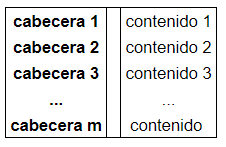
\includegraphics[width=\textwidth]{imaxes/g-analisis/region-r1}
        \caption{Región R1}
        \label{fig:region-r1}
    \end{subfigure}
    \hfill
    \begin{subfigure}[b]{0.65\textwidth}
        \centering
        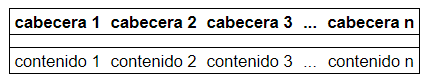
\includegraphics[width=\textwidth]{imaxes/g-analisis/region-r2}
        \caption{Región R2}
        \label{fig:region-r2}
    \end{subfigure}
    \caption{Estructura de dos de los tipos de regiones habituales}
    \label{fig:tipos-de-regiones}
\end{figure}

Un caso especial son las tablas bidimensionales donde se necesita utilizar la Transformada de Hough. Tendrán el código \verb|T2| en las plantillas y por lo demás son similares a las \verb|T1|.

En los documentos de OVH, dado que las tablas no tienen una longitud fija, se consideran en su lugar las relaciones entre las propias tablas y la página en la que se encuentran u otros elementos fijos, como la línea del final, mencionada anteriormente. En las plantillas definirán regiones contiguas, por ejemplo, \verb|T2_T2|. Esto indicará al generador de código intermedio que esta región aplica siempre y cuando se encuentre dos regiones \verb|T2| anexas.

Como conclusión, es de esperar que el tipo de regiones diferentes crezca según se incorporan más y más modelos al sistema. Pero, al mismo tiempo, dado que los tipos de regiones representan un concepto general y son aplicables a cualquier modelo, el objetivo es que su número tienda a estabilizarse con el tiempo.

% TODO aumentar explicación de los tipos de regiones en OVH

\subsection{Características para la identificación}

Para emparejar los documentos con las plantillas que los resuelven se identifican datos específicos presentes en modelos. Dado que todos los casos son facturas, necesariamente aparecerá en ellas el NIF o CIF del emisor. Esta información será suficiente para la identificación. Los mecanismos empleados para realizar el emparejamiento se explican en la Subsección \ref{subsec:impl-identificacion}.

